\subsection{Original evidence and motivation for the follow-up}

The original campaign retained 300 completed drain trials, 60 completed serial trials, 59 completed publication trials and the failed D038 outcome. All 120 active recoveries completed; ten plain-read controls remained pending. Detailed original results and attempt accounting are in Appendix~\ref{app:history}.

At $\Delta=250$ ms, kills at 10\%/75\% of the receipt-based interval were followed by median delays of 226.5/63.6 ms for JetStream and 230.2/67.9 ms for Redis's 10 ms reclamation sleep. Redis's 100 ms sleep raised the late-kill median to 134.0 ms. These observations motivate matched live controls and the current CLAIM arm. Increasing consumers from one to sixteen raised original mean drain throughput by 8.59--12.94 times across profiles, with higher cycle p99. Every recorded worker interval satisfied Equation~\ref{eq:occupancy}. The always-profile rates concern different consumer-progress persistence contracts.

Original periodic/memory publication ratios were approximately 0.8305 for Redis and 0.8197 for JetStream. Always-mode means were 3028 msg/s for nine completed Redis trials and 375 msg/s for ten JetStream trials. Their fixed-count, one-publisher means were 603 and 585 msg/s, respectively. Unequal storage history, mismatched serial duration, missing D038 timings and influential tail observations prevent a causal interpretation of these contrasts. The fresh-store experiments address selected weaknesses while preserving all historical outcomes.

\subsection{Follow-up outcomes and evidence quality}

All 612 planned outcomes were collected: 601 procedures completed and eleven publication trials failed (Table~\ref{tab:followup-outcomes}). Failures were concentrated in always profiles: ten of 72 planned attempts (13.9\%), comprising four warm-up failures and six measurement-stage failures. Periodic profiles had one failure among 72 attempts (1.4\%), in historical JetStream; memory profiles had none among 72. Table~\ref{tab:publication-profile-failures} separates the stages. These are observed fractions of the balanced planned configuration matrix, not estimates of a universal operational failure probability.

The seven timed failures retain 14651 confirmed and 22 unknown request records. Four trials ended with Redis socket I/O timeout errors and three with NATS response timeouts. Recorded unknown-call durations ranged from 5.000 to 5.002 s; the sixteen-publisher JetStream failure retained sixteen unknown requests, so a failed trial need not represent a single failed call. A timeout records the client returning without confirmation, not the time at which the broker completed or abandoned the operation. Warm-up failures have no timed trace and cannot be counted as fifteen-second measurement windows. Appendix~\ref{app:followup-failures} preserves each failure, its error class, and the distinction between client confirmations and later non-atomic inventories. No successful-workload throughput is imputed for a failed attempt.

\begin{table}[htbp]
\centering\small
\begin{tabular}{lrrrrr}
\toprule
Profile & Planned & Complete & Warm-up & Timed & Failed, \%\\
\midrule
Memory & 72 & 72 & 0 & 0 & 0.0\\
Periodic & 72 & 71 & 0 & 1 & 1.4\\
Always & 72 & 62 & 4 & 6 & 13.9\\
\bottomrule
\end{tabular}

\caption{Publication outcomes by append profile across both versions, publisher counts and all deployments. Warm-up and Timed count failures in those stages. Failure percentages use all 72 planned attempts per profile; warm-up failures never enter the timed publication phase.}
\label{tab:publication-profile-failures}
\end{table}

Event reconstruction checked 80263171 timed records, including those unknown outcomes. All 349 completed publication, drain and diagnostic workloads passed stored-ID and full-payload comparison. These are recorded runtime checks and offline consistency checks, not independent experimental replication or a storage-fault test. No completed slow observation was removed, and no failed primary cell was replayed into success.

\begin{table}[htbp]
\centering\small
\begin{tabular}{lrrr}
\toprule
Family & Planned & Complete & Failed\\
\midrule
Publication & 216 & 205 & 11\\
Drain & 96 & 96 & 0\\
Recovery & 252 & 252 & 0\\
Trace & 24 & 24 & 0\\
Compression & 24 & 24 & 0\\
\bottomrule
\end{tabular}

\caption{All planned follow-up outcomes across three deployments. A complete negative control means that the observation procedure completed with the message still pending. Failed trials remain outcomes and do not receive invented successful-workload metrics.}
\label{tab:followup-outcomes}
\end{table}

\subsection{RQ1: live controls and current reclamation policies}

All 120 killed-victim and 120 live-unacknowledging episodes redelivered the original identifier and cleared pending state. At every fixed policy, threshold, victim state and deployment, the later reference age had a shorter mean reference-to-redelivery interval. No receipt preceded the reference event; the largest kill-invocation-to-exit bracket was 2.23 ms. Live redelivery confirms that consumer death is not a necessary trigger in these configurations.

Figure~\ref{fig:followup-recovery} separates the timeout from receipt-based excess. Across deployment-specific condition means, XAUTOCLAIM excess ranged from 0.98 to 10.70 ms and JetStream excess from 1.62 to 9.80 ms. Current Redis CLAIM ranged from 20.52 to 87.83 ms under its 100 ms blocking-read policy. Its paired killed-minus-live differences ranged from $-26.91$ to 14.64 ms, precluding an equivalence claim from close overall averages. These are joint broker/client policy observations, not an intrinsic recovery-speed ranking or directly observed server-timer delays.

All twelve plain-read controls retained pending state without redelivery. Their recorded reference-to-survivor-completion times ranged from 0.503 to 0.699 s for a nominal 0.500 s budget. The follow-up therefore reports actual endpoints, while the original controls retain only their nominal-budget interpretation.

\begin{figure}[htbp]
\centering
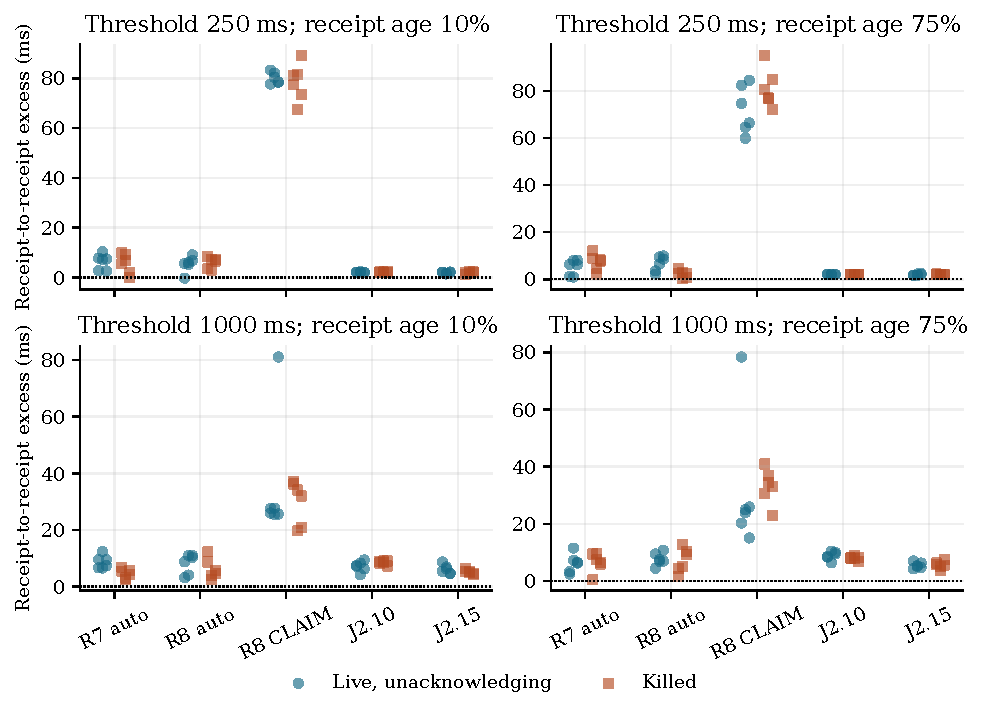
\includegraphics[width=\linewidth]{figures/followup-recovery.pdf}
\caption{Every active follow-up recovery episode, showing receipt-to-receipt time minus the configured eligibility threshold. Blue circles are live, deliberately unacknowledging victims; orange squares are killed victims. Horizontal offsets separate deployments and do not encode time. R7/R8 denote Redis 7.4.2/8.10.2; auto denotes XAUTOCLAIM with a 10 ms sleep; J denotes JetStream. Zero is a client-receipt reference, not a verified broker-side lower bound.}
\label{fig:followup-recovery}
\end{figure}

\subsection{RQ2: consumer scaling and driver capacity}

All 96 follow-up drains completed. Across deployment-specific paired comparisons, sixteen consumers raised mean throughput by 10.43--14.49 times relative to one consumer in the current memory/periodic profiles. Mean trial cycle p99 increased in all eight engine/profile/driver-quota conditions. The 65536-message drains lasted 1.77--30.11 s, extending the shortest high-concurrency observations beyond the original subsecond runs while remaining finite workloads.

At sixteen consumers, changing the driver from two to four CPUs, with matching GOMAXPROCS, produced mean paired throughput ratios of 1.031/1.026 for Redis memory/periodic and 1.107/1.102 for JetStream. Redis-periodic deployment ratios ranged from 0.993 to 1.048, so the direction was not uniform. No driver or broker cgroup throttling was recorded within the 96 bracketing drain samples. The increased rates and changed cycle tails nevertheless show that absence of throttling alone cannot establish that driver configuration is irrelevant. Table~\ref{tab:followup-drain} reports the corresponding CPU use; these observations concern the combined client, protocol and broker path.

\begin{table}[htbp]
\centering\small\setlength{\tabcolsep}{3pt}
\begin{tabular}{llrrrlrr}
\toprule
System & Mode & CPU & $X_1$ & $X_{16}$ & $X_{16}/X_1$ & Driver & Broker\\
\midrule
Redis & M & 2 & 2.83 & 34.98 & 12.36 [12.02, 12.86] & 1.08 & 0.56\\
Redis & M & 4 & 2.85 & 36.05 & 12.68 [12.21, 13.52] & 1.43 & 0.56\\
Redis & P & 2 & 2.59 & 28.55 & 11.05 [10.43, 11.73] & 0.98 & 0.64\\
Redis & P & 4 & 2.55 & 29.31 & 11.48 [11.34, 11.61] & 1.32 & 0.64\\
JetStream & M & 2 & 2.28 & 29.54 & 12.98 [12.62, 13.34] & 1.11 & 1.29\\
JetStream & M & 4 & 2.28 & 32.67 & 14.32 [14.14, 14.49] & 1.50 & 1.35\\
JetStream & P & 2 & 2.26 & 28.70 & 12.72 [12.61, 12.79] & 1.11 & 1.28\\
JetStream & P & 4 & 2.28 & 31.62 & 13.89 [13.84, 14.00] & 1.47 & 1.34\\
\bottomrule
\end{tabular}

\caption{Current-release drain results. CPU is the driver's configured quota; $X_1$ and $X_{16}$ are throughput in kmsg/s. Point values equally weight campaign means. The speedup column gives the mean and range of campaign-specific paired ratios. Driver/Broker are mean CPU cores used during the bracketing samples at $C=16$, not percentages. M/P denote memory/periodic.}
\label{tab:followup-drain}
\end{table}

\subsection{RQ3: confirmed publication from fresh stores}

At sixteen publishers, equal-weight deployment means for Redis 8.10.2 were 73.26, 60.49 and 4.35 kmsg/s in memory, periodic and always profiles. JetStream 2.15.0 yielded 60.62, 49.75 and 0.565 kmsg/s. Each condition completed all nine planned trials except JetStream always, with eight completions. The paired periodic/memory ratios averaged 0.8257 for Redis and 0.8207 for JetStream, with deployment ranges 0.8082--0.8397 and 0.8091--0.8296; all nine pairs were available in each comparison. These are configured confirmation costs from the specified starting procedure.

The latency trade-off remains visible. For memory, periodic and always profiles, respectively, mean trial p99 at sixteen publishers was 0.470, 0.563 and 16.98 ms for current Redis, and 0.639, 0.796 and 295.64 ms for current JetStream. A retained JetStream-always trial, main03/F0039, contained 976 confirmations and a 1968.6 ms p99, with nine higher order-statistic positions. Its tail remains part of the result. Appendix~\ref{app:followup} reports every condition's completion and sample counts; these empirical tails do not establish stable production percentiles.

Long requests also occurred in completed trials. Seven completed always-profile trials had a confirmed-request maximum of at least 1000 ms, spanning both brokers and both versions. Four exceeded 2000 ms, with maxima from 2.297 to 4.183 s; the next-highest maximum was 1.969 s. Appendix~\ref{app:request-maxima} lists all seven cases. These thresholds are post-observation descriptive summaries, not prospective exclusion rules or production tail guarantees. Together with the timeout outcomes, they show operationally material latency variation that is not represented by completed-run mean throughput alone.

Matched publication durations clarify the concurrency comparison that the original serial sensitivity could not isolate. For current Redis always mode, the mean paired sixteen/one-publisher ratio was 9.41, ranging from 6.06 to 13.67 across deployments, using six of nine planned pairs. Current JetStream's corresponding mean was 1.55, ranging from 0.73 to 2.46, using seven pairs. More publishers therefore did not improve every deployment's always-mode mean. Neither current release nor fresh storage removes all observed long requests or timeout outcomes. Across the eight memory/periodic version contrasts at one and sixteen publishers, equal-weight means of the deployment-specific current/historical ratios ranged from 0.9603 to 1.0232, within approximately 4\% of unity. Individual deployment ratios ranged more widely, from 0.9401 to 1.1237. All contrasts used nine completed pairs except JetStream periodic at one publisher, with eight. Appendix~\ref{app:version-contrasts} gives the individual condition summaries. These descriptive comparisons do not establish version equivalence.

\begin{figure}[htbp]
\centering
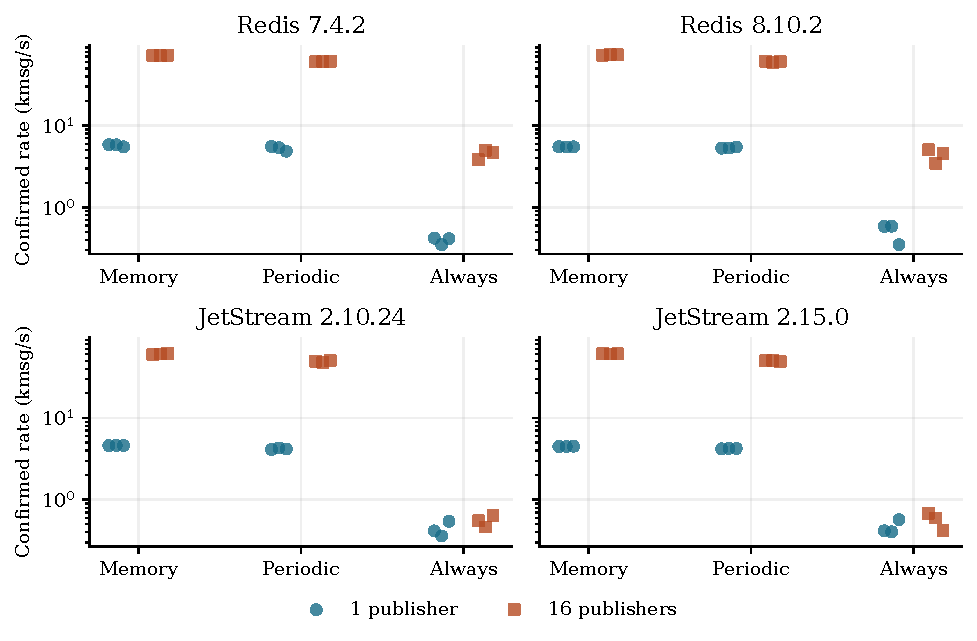
\includegraphics[width=\linewidth]{figures/followup-publication.pdf}
\caption{Fresh-store publication with matched 15-second admission budgets. Each point is one deployment's mean over completed planned trials of that condition. Horizontal offsets separate deployments; they have no quantitative meaning. The vertical scale is logarithmic. Failure counts and all per-deployment values accompany the results in Appendix~\ref{app:followup}.}
\label{fig:followup-publication}
\end{figure}

\subsection{Synchronization and compression diagnostics}\label{sec:followup-diagnostics}

All 24 trace-family and 24 compression-family trials completed. In the twelve instrumented trials, the broker-side phase brackets contained no synchronization-call errors or boundary-overlapping calls. The synchronization-call/confirmation ratio was 1.000 for current Redis with one publisher and approximately 0.120 with sixteen. Current JetStream's ratio was 1.000 at both publisher counts. JetStream's one-call-per-confirmation count at both publisher counts is consistent with serialized per-message synchronization in the tested single-stream append path: the pinned file store holds its write lock while storing a message, and its always-mode flush invokes synchronization before returning~\cite{nats2150filestore}. Redis's concurrent aggregate ratio corresponds to approximately 8.3 confirmations per synchronization call, supporting shared synchronization across publications. This identifies a source-consistent contributor to the different concurrency response; it does not assign every confirmation to an individually traced call, measure physical device flushes, or decompose the entire cross-system performance gap.

Tracing reduced throughput. Mean traced/plain ratios at one and sixteen publishers were 0.943 and 0.815 for Redis, and 0.920 and 0.934 for JetStream, respectively. Within-trace call p99 values ranged from 2.00 to 2.76 ms, and the largest traced synchronization call lasted 544.6 ms. These separate diagnostic samples did not capture the untraced primary timeout events or main03/F0039's much larger request tail, and they do not establish the cause of those events.

Disabling inherited compression produced mean off/inherited ratios of 1.036/0.995 for Redis filler/template payloads and 1.021/0.988 for JetStream. All twelve deployment-specific ratios lay between 0.935 and 1.063, with both directions represented. The complete table is in Appendix~\ref{app:followup}. This sensitivity does not support attributing the large always-mode gap to compression alone; it does not establish that compression or Btrfs is irrelevant under other conditions.

\begin{table}[htbp]
\centering\footnotesize\setlength{\tabcolsep}{3pt}
\begin{tabular}{lrllllr}
\toprule
System & $P$ & Sync calls & Calls/msg & Call p99, ms & Traced/plain & $n_t/n_p$\\
\midrule
Redis & 1 & 8327 [8233, 8427] & 1.000 [1.000, 1.000] & 2.31 [2.23, 2.42] & 0.94 [0.91, 0.97] & 3/3\\
Redis & 16 & 7349 [7270, 7392] & 0.120 [0.120, 0.121] & 2.51 [2.24, 2.76] & 0.82 [0.79, 0.84] & 3/3\\
JetStream & 1 & 7797 [7728, 7860] & 1.000 [1.000, 1.000] & 2.48 [2.23, 2.66] & 0.92 [0.90, 0.96] & 3/3\\
JetStream & 16 & 9644 [9481, 9762] & 1.000 [1.000, 1.000] & 2.33 [2.00, 2.60] & 0.93 [0.92, 0.95] & 3/3\\
\bottomrule
\end{tabular}

\caption{Current always-profile synchronization diagnostics. Entries give the mean and range of available deployment estimates; $n_t/n_p$ counts complete traces/paired comparisons, each out of three. Call p99 is a within-trace order statistic. Traced/plain is the paired throughput ratio. Counts combine fsync and fdatasync inside the broker's phase brackets; they are not physical device-flush counts.}
\label{tab:followup-trace}
\end{table}


\FloatBarrier

